	\subsection{2.15. Диаграммы МО для электронодефицитных соединений.} 
	
	\par\bigskip
	
	\begin{figure}[H]
		\centering
		{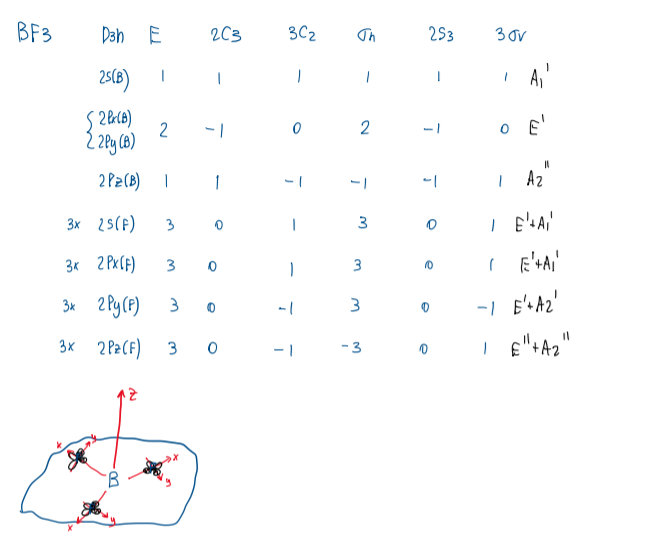
\includegraphics[scale=1]{38.png}}
	\end{figure}
	
	\begin{figure}[H]
		\centering
		{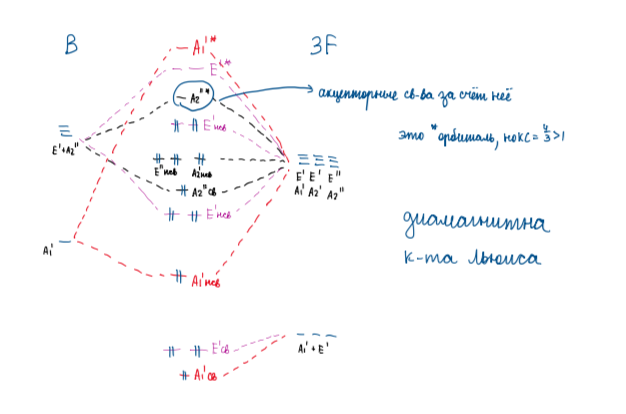
\includegraphics[scale=1]{39.png}}
	\end{figure}

\begin{figure}[H]
	\centering
	{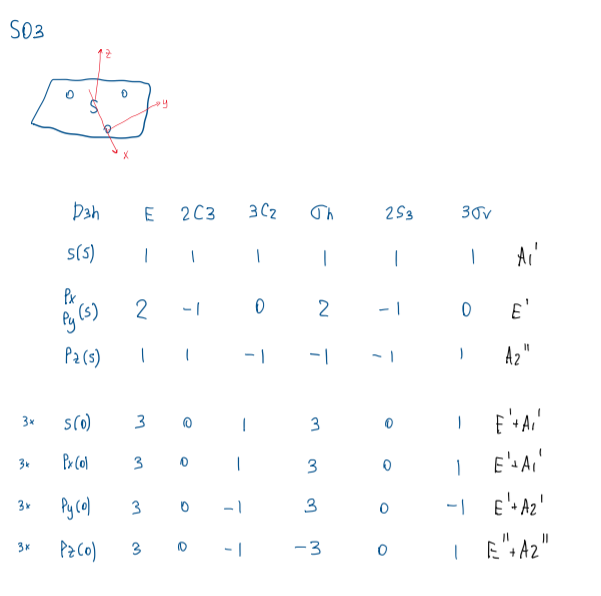
\includegraphics[scale=1]{40.png}}
\end{figure}

	\begin{figure}[H]
		\centering
		{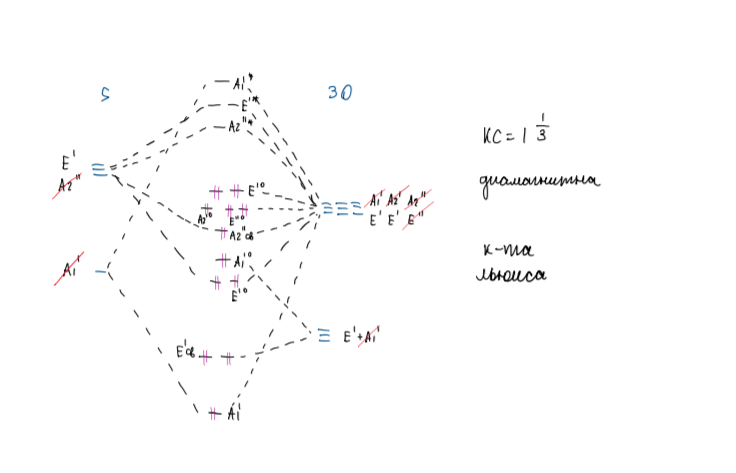
\includegraphics[scale=1]{41.png}}
	\end{figure}
	
	Выше приведены примеры МО для двух различных
	электронодефицитных соединений. Из МО следует
	акцепторная природа таких соединений: акцептирование
	будет происходить на разрыхляющую орбиталь А2’’, это
	позволяет сделать КС>1. Отдача электронных пар с
	несвязывающих орбиталей Е’ не характерна, поскольку они
	локализуются довольно близко к
	высокоэлектроотрицательным элементам - фтору и
	кислороду соответственно. В рамках трёхцентрового
	двухэлектронного взаимодействия (3с2е) образуются три
	вида молекулярных орбиталей (на примере $SO_3$):
	
	\begin{figure}[h]
		\centering
		{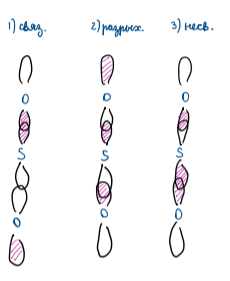
\includegraphics[scale=1]{42.png}}
	\end{figure}
	
	Благодаря диаграмме МО для $SO_3$ мы можем сделать важный
	вывод. Заметим, что часто рисуют $SO_3$ с тремя двойными связями к
	атомам кислорода. На самом деле, такое изображение не очень
	корректно, ведь у серы будет целых 12 электронов. Из диаграммы
	МО следует, что реально в связывании принимают только три
	орбитали серы, а одна р-орбиталь остается пустой. Взаимодействие
	же с ней р-орбиталей кислорода второстепенно, им можно
	пренебречь. Получается, более правильным рисунком будет
	рисунок внизу, где есть три донорно-акцепторные связи, и от этого
	степень окисления серы не изменится.
	
	\begin{figure}[H]
		\centering
		{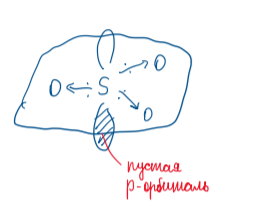
\includegraphics[scale=1]{43.png}}
	\end{figure}
	
	\par\bigskip
	\par\bigskip
	